\documentclass[apj]{aastex}
\shorttitle{Delay Time Distributions of SNe~Ia}
\shortauthors{Strolger et al.}

\usepackage{natbib}
\usepackage{nicefrac}
\usepackage{ulem}
\usepackage{xcolor}
\usepackage{amssymb,amsmath}
\bibliographystyle{apj}

\renewcommand{\deg}{^{\circ}}
\begin{document}
\title{The Empirical Delay Time Distributions of Type Ia Supernovae From Galaxy Star Formation Histories}
\author{L.-G.~Strolger, Pacifici, Rodney, et al.}

\begin{abstract}
blah, blah, blah \ldots
\end{abstract}

\clearpage

\section{Introduction}
There have been several measures of the volumetric SN~Ia rate at various redshifts by various groups. These rate values have not always been in total agreement with one another, and there may be several valid reasons as to why (see rev. by Haden?). But as there is little concession on which is the most appropriate way to express measures in event rates, it it probably best to consider each as a valid measure. Further, we assume each is valid within their measured statistical error, which again may be bold, but is probably satisfactory given the number of rate measures in each redshift interval.

\begin{figure}[t]
   \centering
   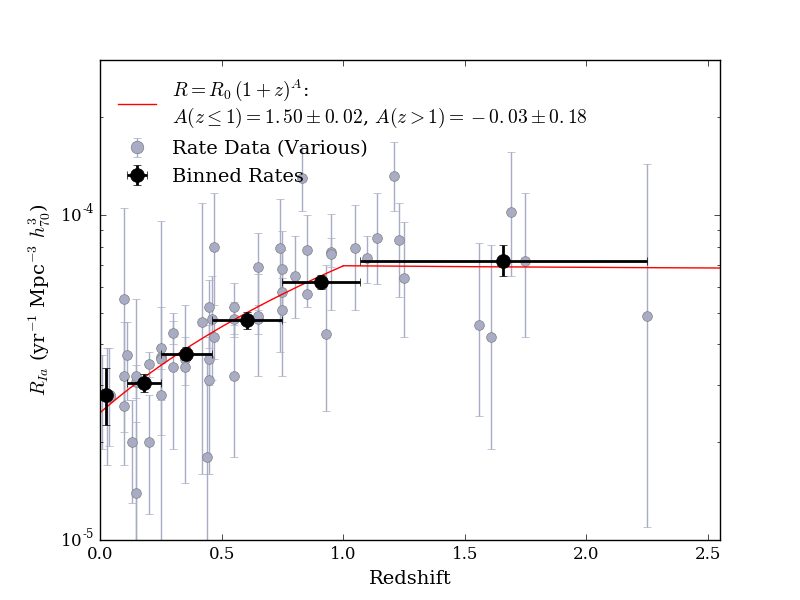
\includegraphics[width=6.1in]{figure_SNIa_rate_z_pwr_fit}
   \caption{\footnotesize Type Ia supernova volumetric rate measures from various sources in the literature (gray points, also see Table), and binned (black points) for illustration. Red lines show a broken power-law fit to the data in redshift space.}
   \label{fig:sn1a_rates}
\end{figure}

It would be reasonable to assume the volumetric rates follow a broken power law evolution with redshift, i.e., $R_{Ia}=R_0\,(1+z)^A$ where at $z<1$ the power-law slope is $A=1.50\pm0.02$ (with $R_0 = 2.5\pm0.2\times10^{-5}$ yr$^{-1}$ Mpc$^{-3}$ $h_{70}^3$), which flattens substantially to $A=-0.03\pm0.2$ at redshifts greater than 1 (see Figure~\ref{fig:sn1a_rates}). 

For these types of analyses, the standard assumption is that the stellar death rate (or supernova rate) is related to the stellar birth rate, convolved with some delay-time distribution that contains all the temporal factors of stellar evolution (e.g., main sequence lifetime, etc.) and binary star evolution (e.g., accretion rates or merger times). Two additional terms include the fraction of the initial mass function (or IMF) that are the progenitors to the SNe~Ia (presumably $3 - 8\, \rm{M}_{\odot}$ zero-age main sequence stars), and the fraction of that population that are actually capable of producing events, as not are necessarily in the right type of binary system or systems.

We can relate volumetric SN~Ia rate history to the cosmic star formation history($\dot{\rho}_{\star}$) in a similar way, expressed mathematically by, 
\begin{equation}
%R_{Ia}(t) = k\varepsilon\int_0^t \dot{\rho}_{\star}(\tau) \ast \Phi(t' - \tau)\,dt',
R_{\rm Ia}(t) = k\,\varepsilon\,\biggl[\dot{\rho}_{\star}(t) \ast \Phi(t)\biggr],
\label{eqn:std}
\end{equation}
\noindent where $\Phi(t)$ is the delay-time distribution of SNe~Ia, $k$ is the fraction of the IMF (by mass) responsible for SN~Ia progenitors, $\varepsilon$ is the fraction of that population that are ultimately successful in producing SNe~Ia, and $t$ is the forward-moving clock of the universe. 

\subsection{The fraction of stars responsible for SNe~Ia}
Dissecting each of these terms, $k$ is perhaps the easiest to approximate. The progenitors of SNe~Ia have traditionally been CO WD which acquire sufficient mass to approach or exceed the Chandrasekhar mass limit, $M_{ch}=1.44\,M_{\odot}$. To only marginally achieve this, they can either start at sufficiently high mass to require only a small amount of accretion from a nearby companion (typically single-degenerate, or SD, scenarios), or as a pair of WD that have a combined mass that meets this criterion (the double-degenerate, or DD, scenario) setting an even lower constraint~\cite[see][for a review]{Maoz:2013}. In the case of WD/WD mergers, WD mass distributions are strongly peaked around $M_{WD}\approx0.6\pm0.1\,M_{\odot}$ \citep{Catalan:2008il}, in which a pair drawn from such distribution may be satisfactorily close to the ignition threshold of a carbon core for a nonrotating CO WD, approximately $1.38\, M_{\odot}$ of \cite{Arnett:1969dw} and \cite{Nomoto:1982vh}. Initial-Final Mass relations \cite[e.g.,][]{Catalan:2008il,Cummings:2018oe} would correspond these to ZAMS masses of approximately $3\, M_{\odot}$, but no less than $\sim2.5\, M_{\odot}$. 

The same Initial-Final Mass relations would suggest that WD essentially at $M_{ch}$ would fall just below $8\, M_{\odot}$ ZAMS. On a more physical bases, simulations show that the lowest mass in which C ignition is still possible is around $6-8 \,M_{\odot}$~\cite{Chen:2014rb,Denissenkov:2015rf}, but likely no more than $\sim11\, M_{\odot}$ \citep{Takahashi:2013jx}, above which an electron-capture-induced collapse mechanism begins, marking the onset of core-collapse supernovae.

It is reasonable, therefore, to assume a progenitor mass range of about $3-8\,M_{\odot}$ ZAMS. From a numerical assessment of these stars, assuming they fall within an IMF that is a power-law distribution by mass (in this initial mass range) with $\alpha\approx-2.3$~\citep{Salpeter:1955rw,Kroupa:2001gf}, one would expect 
\begin{equation}
k = \frac{\int\limits_{3M_{\odot}}^{8M_{\odot}} \xi(M)\,dM}{\int\limits_{0.1M_{\odot}}^{125M_{\odot}} M\,\xi(M)\,dM},
\end{equation}
\noindent where $k = 0.021^{+33\%}_{-24\%}\,M_{\odot}^{-1}$. The error in $k$ is driven more by choices in the upper and lower value in the selected mass range of  SN~Ia progenitors than by the choice in IMF model, as described above.

The fraction of CO WDs that are successful in making SNe~Ia is hard to determine, as we don't quite yet know the details of the progenitor mechanism or mechanisms. Estimates swing rather wildly from (perhaps) from as low as 1 in 200~\citep{Breedt:2017rp} to as optimistic as 1 in 40~\citep{Maoz:2012}. There is at least strong consensus that accretion on to a CO WD is essential, but very different plausible WD close binary scenarios from at least a theoretical standpoint~\citep{Nelemans:2001hb,Nelemans:2001cs}. The binary fractions of WDs has been recently estimated from the  the ESO-VLT Supernova-Ia Progenitor Survey~\citep[SPY]{Napiwotzki:2007} show close double WD systems may have $\varepsilon_{\rm bin}\simeq0.1\pm20\%$, with separations distributed following a power-law slope of $\alpha=-1.3\pm15\%$~\citep{Maoz:2017zl}. It is not likely all of these successfully yield SNe~Ia as their merger rates in the MW are at least a magnitude higher than best estimates of the SN~Ia rate in our galaxy, and presumably some of these will form AM CVn and R Corona Borealis stars, but at least it could be treated as an upper limit on $\varepsilon$.

\subsection{The star-formation density history}
The cosmic star formation history (CSFH), at least to $z < 5$, or over 90\% of the history of the universe, is fairly well understood, with~\cite{Madau:2014fk} providing one of the most complete compilations. However there is significant scatter in individual tracers of the compilation, as some are provided from limited probed volumes leading to large uncertainties in fluctuations with cosmic variance. The CSFH data derived recently from the combined GAMA, G10-COSMOS, and 3D-HST datasets by~\cite{Driver:2018nr} is alternatively done in a quasi-homogeneous analysis over a larger area, leading to greatly reduced total uncertainties. The derived trend is somewhat consistent with ~\cite{Madau:2014fk}, but has a notably weaker peak at `cosmic noon' ($z\sim2$) and a slower build-up of unobscured star-formation at high-$z$ (see Figure~\ref{fig:csfhs}).
Using the parameterization in \cite{Madau:2014fk}, where
\begin{equation}
\dot{\rho}_{\star}(z) = \frac{A\,(1+z)^C}{((1+z)/B)^D+1}.\label{eqn:mdp}
\end{equation}
\noindent We fit the above function to MD14 data using a Levenberg-Marquardt least-squares algorithm, resulting in the solid blue line and error region shown in Figure~\ref{fig:csfhs}, with $A=0.013\pm0.001$, $B=2.6\pm0.1$, $C=3.2\pm0.2$, and $D=6.1\pm0.2$, slightly different from the values fit in MD14. The same functional fit to the \cite{Driver:2018nr} data yields $A=0.009\pm0.001$, $B=2.7\pm0.5$, $C=2.5\pm0.4$, and $D=4.1\pm0.3$.

\begin{figure}[t]
   \centering
   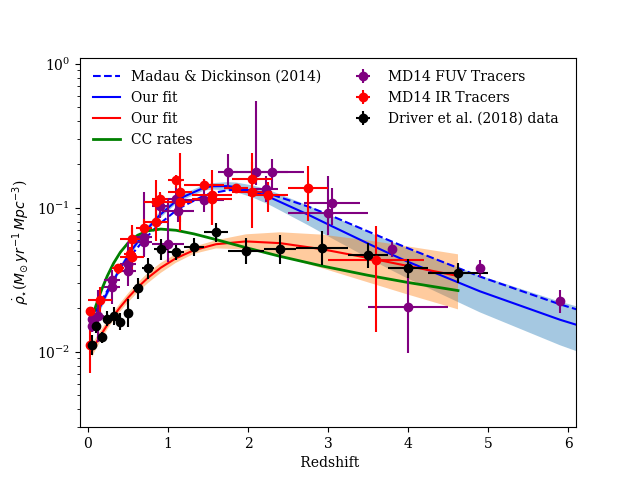
\includegraphics[width=6.1in]{figure_csfh_today}
   \caption{\footnotesize Shown are the compendium cosmic star formation histories, from ~\cite{Madau:2014fk} and ~\cite{Driver:2018nr}. Lines are fits to the data as indicated, and shaded regions represent the 1-$\sigma$ confidence intervals to the fits. Also shown for comparison is the model fit to core-collapse SN rates from~\cite{Strolger:2015aa}.}
   \label{fig:csfhs}
\end{figure}
\noindent [NOTE: more on which is the better choice, or if analysis on the end should be done on both.]



\subsection{SN~Ia progenitor delay times}
\noindent [NOTE: talk about the expected delay-time distribution, values from Graur and Maoz, inability to probe turnover at `SN high noon', around $z\sim1$.]

\begin{figure}[t]
   \centering
   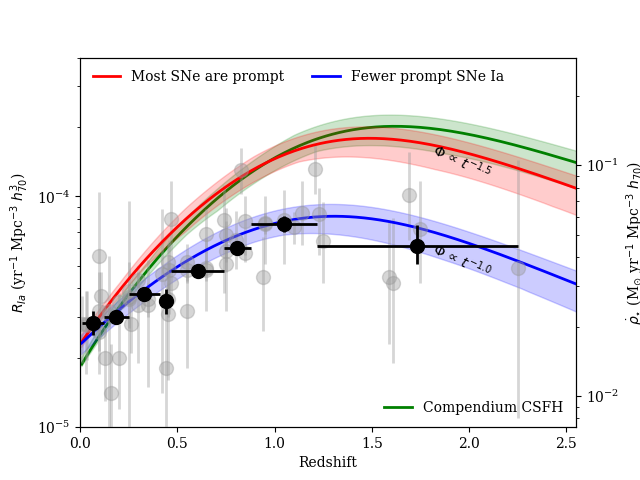
\includegraphics[width=6.1in]{figure_SNIa_rate_alpha}
   \caption{\footnotesize Shown in comparison to the data are the expected volumetric rates for power-law delay-time distributions ($\alpha = 1.0$ and 1.5 in red and blue, respectively) as applied to the cosmic star formation rates~\cite[in  solid and dashed green, respectively]{Madau:2014fk,Driver:2018nr}. Dashed rate models require a higher fraction of WD progenitors than the solid lines.}
   \label{fig:sn1a_rates2}
\end{figure}

Following \cite{Strolger:2010}, we can continue to test a robust delay-time model, capable of reproducing the theoretical distributions for SD and DD models at one extreme, and $\delta$-function delay times at the other. The unimodal, skew-normal $\Phi(\tau)$ function is defined as:

\begin{equation}
	\Phi(\tau)=\frac{1}{\omega\pi}\,\exp\biggl(\frac{-(\tau-\xi)^2}{2\omega^2}\biggr)\int_{-\infty}^{\alpha (\frac{\tau-\xi}{\omega})} \exp\biggl(\frac{-t'^2}{2}\biggr)\,dt',
\label{eqn:model}
\end{equation}

\noindent where location ($\xi$),\footnote{Different from the initial mass function, $\xi(M)$.} width ($\omega^2$), and shape ($\alpha$) define the mode time ($\bar{\tau}$), variance ($\sigma^2$), skewness ($\gamma_1$), and kurtosis ($\gamma_2$) of the model function by,

\begin{eqnarray*}
\bar{\tau}&=&\xi+\omega\delta\sqrt{\frac{2}{\pi}},\\
\sigma^2&=&\omega^2\biggl(1-\frac{2\delta^2}{\pi}\biggr),\\
\gamma_1&=&\frac{1}{2}(4-\pi)\frac{(\delta\sqrt{2/\pi})^3}{(1-2\delta^2/\pi)^{3/2}},\\
\gamma_2&=&2(\pi-3)\frac{(\delta\sqrt{2/\pi})^4}{(1-2\delta^2/\pi)^{2}}.\\
\end{eqnarray*}

where $\delta=\alpha\,(1+\alpha^2)^{-1/2}$. Figure~\ref{fig:dtd_families} demonstrates the flexibility of the model in producing various distributions in $\tau$. 

\begin{figure}[t]
   \centering
   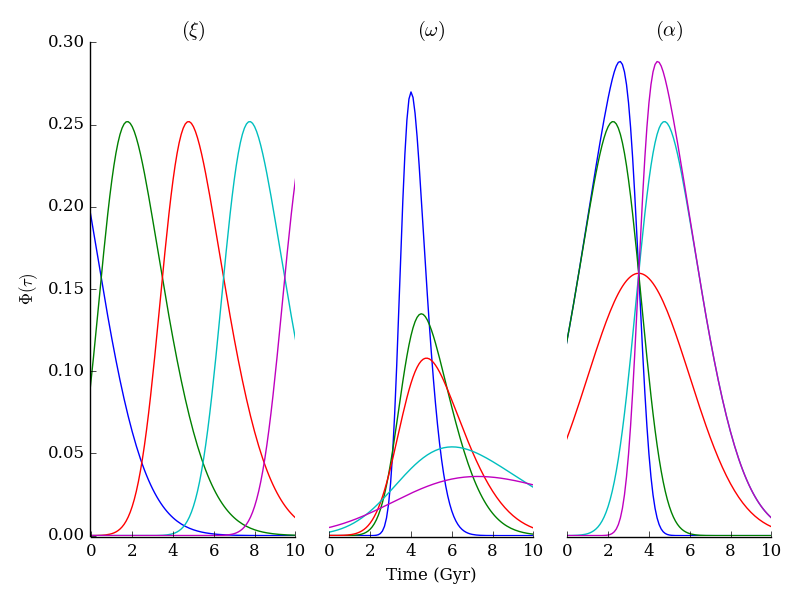
\includegraphics[width=6.5in]{figure_dtd_families}
   \caption{\footnotesize Families of delay-time distributions models shown for various values of location ($\xi$) fixing other parameters (left plot of figure), width ($\omega$, middle plot), and shape ($\alpha$, right plot), for illustration purposes.}
   \label{fig:dtd_families}
\end{figure}

\section{Delay Time Distributions from Volumetric SN~Ia Rates and the Cosmic Star Formation History}

\subsection{The optimized solution}
We apply a maximum likelihood estimation method to determine the best-fit unimodal delay time model to Equation~\ref{eqn:std} using a method described in \cite{Hogg:2010fj} and the {\tt emcee.py} documentation~\citep{Foreman-Mackey:2013pd}. We assume, for simplicity, that the errors of all survey data are gaussian in nature, but may be underestimated by some factor ($f$), which may be correctly justified given we are only using the statistical error produced for each value. 

\begin{figure}[t] %  figure placement: here, top, bottom, or page
   \centering
   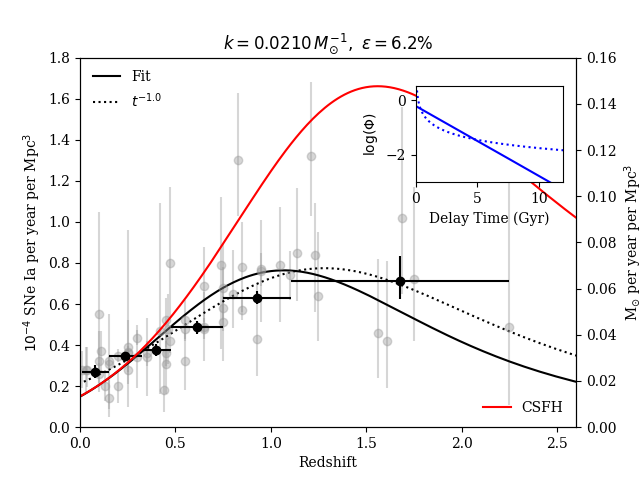
\includegraphics[width=6.5in]{figure_sfd_optimized} 
   \caption{\footnotesize In addition to rate values shown in previous figures, the $R_{\rm Ia}(z)$ result of from optimal parameter fitting is show (black line). The CSFH is shown on in red, and along the secondary abscissa. }
   \label{fig:sfd_optimized_curvefit}
\end{figure}
	
As follows, we adopt the likelihood function to be:
\begin{equation}
\ln p(y|x, \sigma, \varepsilon, \xi, \omega, \alpha, f) = -\frac{1}{2} \sum_i \biggl\{ \frac{[R_{{\rm Ia},i} - {\rm model}(t_i; \varepsilon, \xi, \omega, \alpha)]^2}{s_i^2}+\ln (2\pi s_i^2)\biggr\},
	\label{eqn:lf}
\end{equation}
where,
\begin{equation}
s_i^2 = \sigma_i^2+f^2\, {\rm model}(t_i; \varepsilon, \xi, \omega, \alpha)^2.
\end{equation}
We then find the optimal parameters which maximize this likelihood.

As for priors, we apply rather loose, arbitrary bounds on the optimization, in that we require the successful fraction of progenitors to be between zero and 1, that the width parameters can only be positive, and the that underestimation fraction can only be between zero and 1. Otherwise, the bounds are as follows for parameters $\varepsilon$, $\xi$, $\omega$, $\alpha$, and $\ln f$, respectively: [(0.,1.0),(-2000.,2000.),(0.001,100.),(-500.0,500.0),(-4.,0.)]. The results of that fit are shown in Figure~\ref{fig:sfd_optimized_curvefit}, and in Table~\ref{tab:results}. 


\begin{table}
    \centering
    \caption{Results for unimodal model}
    \label{tab:results}
    \begin{tabular}{cccccc}
        \hline
                Model test & $\varepsilon$ & $\xi$ & $\omega$ & $\alpha$ & $\log f$ \\ 
                \hline
		CSFH Max.~Likelihood &$0.062$&$-1669.7$& $69.1$& $88.7$& $-2.99$\\
                CSFH MCMC & $0.07\pm0.11$ & $-1031^{+1033}_{-687}$ &$65^{+15}_{-20}$& $190\pm210$&  $-2.5^{+0.8}_{-1.4}$\\
                \hline
    \end{tabular}
\end{table}

While the optimization results in values, and a rather interesting delay-time distribution, it is not directly possible to estimate the errors in the parameters via this maximum likelihood optimization method. A Markov chain Monte Carlo (MCMC) is better suited for that.

\subsection{The MCMC solution}
Exploring the parameter space in an MCMC allows both confirmation of the optimized solution and an exploration of the range of validity. We use the affine Invariant MCMC ensemble sampler from {\tt emcee.py}~\citep{Foreman-Mackey:2013pd}, and use the same likelihood function as shown in Equation~\ref{eqn:lf}, and set our uniform priors as described by the bounds, as shown in the previous section. We then set 1,000 walkers to explore 10,000 steps, for a total of 10 million iterations, the first 100,000 of which we discard as `burn-in'. The results of which are shown in Figure~\ref{fig:mcmc_sfd} and Table~\ref{tab:results}.

As is shown, there is a clear convergence in $\ln f$, the factor by which reported errors in rate measures are underestimated. It seems that nearly all values are underestimated by less than 33\%, with most only 10\% underestimated. While there is a large dispersion in rate values, and seemingly inconsistent rates in some of the same redshift ranges, their statistical errors are not grossly underestimated. As fairly well constrained is $\varepsilon$, suggesting (as expected) only $10\pm10\%$ of WD stars contribute as SN~Ia progenitors. That number increases to  $0.14^{+0.13}_{-0.14}$ when the D18 CSFH is used. However, the parameters we wished to know the most about,  $\xi$, $\omega$, and $\alpha$, are very much less constrained by the MCMC. There is a clear peak around $\omega\approx60$, but that value is also highly degenerate with the value of $\xi$.  There does not appear to be any convergence or preference in the value of $\alpha$.

\begin{figure}[t] %  figure placement: here, top, bottom, or page
   \centering
   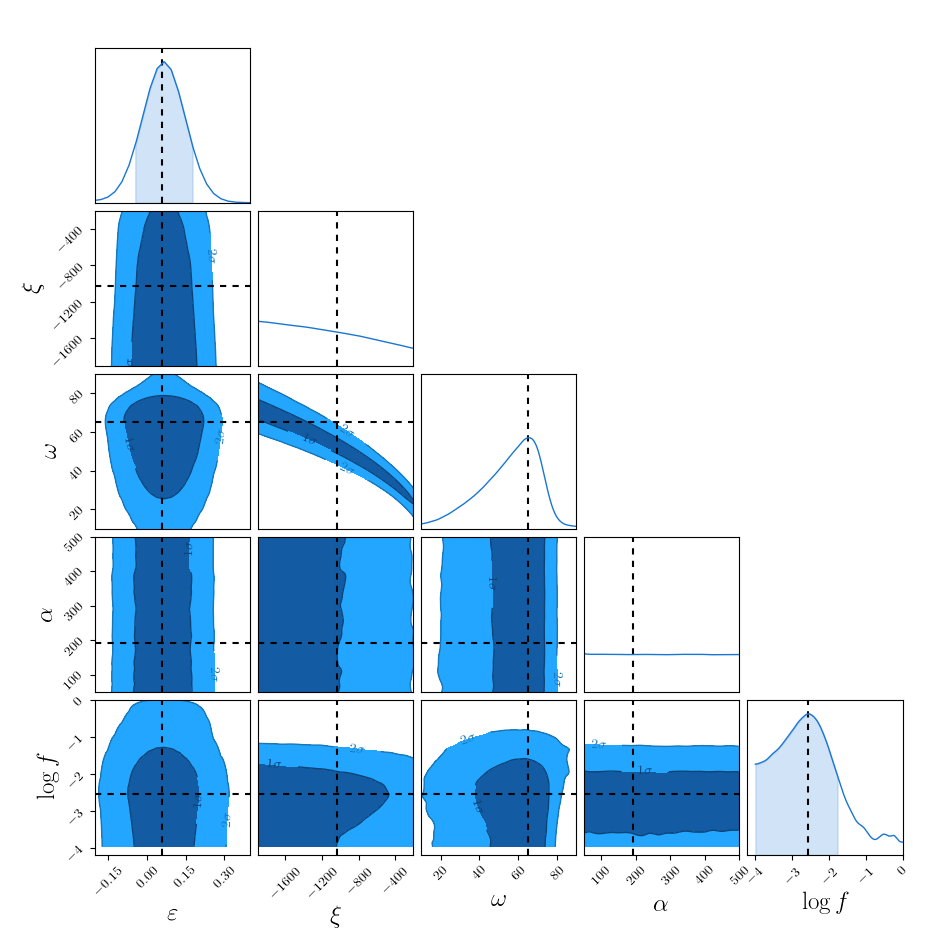
\includegraphics[width=6.5in]{figure_sfd_corners} 
   \caption{\footnotesize MCMC results on unimodal delay-time distribution model, fit to volumetric rate data and CSFH. Plot generated using {\tt ChainConsumer.py} \citep{Hinton:2016qy}.}
   \label{fig:mcmc_sfd}
\end{figure}
\clearpage




\section{Delay Time Distributions from Star Formation Histories}
This is an evaluation of the maximum likelihood delay time distribution following the prescription of \cite{Maoz:2012a} but performed on the GOODS/CANDELS galaxies. In a given galaxy, the total expected rate of SNe~Ia per year will be:
\begin{equation}
R_i = \int_0^t \Psi(t') \ast \Phi(\tau)\,dt'
\end{equation}
\noindent where $\Psi(t)$ is the star formation history of the galaxy (mapped in forward time), and $\Phi(\tau)$ is the delay time distribution model, also forward in time. The product of the integrated rate and the control time, $t'_{c, i}$, which contains all the information on the temporal sampling and depth of the survey, 
\begin{equation}
m_i = R_i \times t'_{c, i}
\end{equation}
\noindent which is the expected number of SN Ia events from that galaxy over the duration of the survey. The probability distribution of observed events is likely Poisson, where of catching $n_i$ SNe~Ia from that galaxy when $m_i$ are expected is
\begin{equation}
P(n_i | m_i) = \frac{m_i^{n_i}e^{-m_i}}{n_i!}.
\end{equation}
The product of probabilities for all galaxies in the survey would then serve as the likelihood of a given delay-time distribution model. The log-likelihood, convenient for MCMCs, is then expressed by:cp 
\begin{equation}
L = \prod _i^N P(n_i|M_i) \Rightarrow \ln L = -\sum^N m_i+\sum^N\ln\biggl(\frac{m_i^{n_i}}{n_i!}\biggr)
\end{equation}
\noindent in which the last term is zero for galaxies which do not host SNe~Ia during the survey.


The model parameters, $\xi$, $\omega$, and $\alpha$ are explored in an Affine Invariant Markov-chain Monte Carlo using {\tt emcee.py} \citep{Foreman-Mackey:2013pd}. As for priors, we restrict the parameters to the space:

\begin{eqnarray*}
-15 <&  \xi &\le 15\\
0 <&\omega &\le 15\\
-15 <&  \alpha &\le 15\\
\end{eqnarray*}


\begin{figure}[t] %  figure placement: here, top, bottom, or page
   \centering
   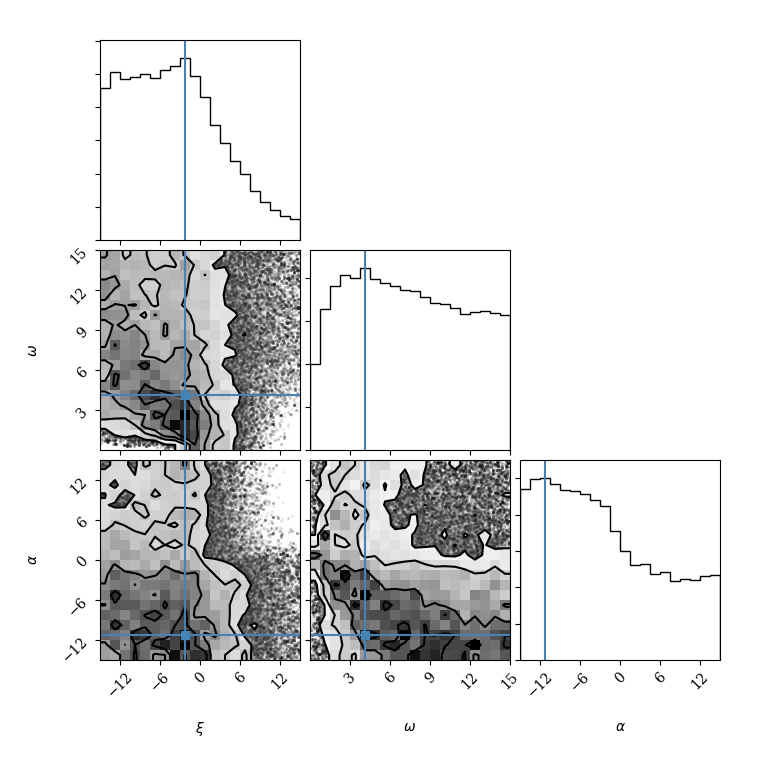
\includegraphics[width=4in]{Figure_1} 
   \caption{\footnotesize MCMC results on 147 galaxies in CANDELS, 49 of which are SN~Ia hosts. Plot generated using {\tt corner.py} \citep{Foreman-Mackey:2016ve}.}
   \label{fig:fg1}
\end{figure}
\begin{figure}[h] %  figure placement: here, top, bottom, or page
   \centering
   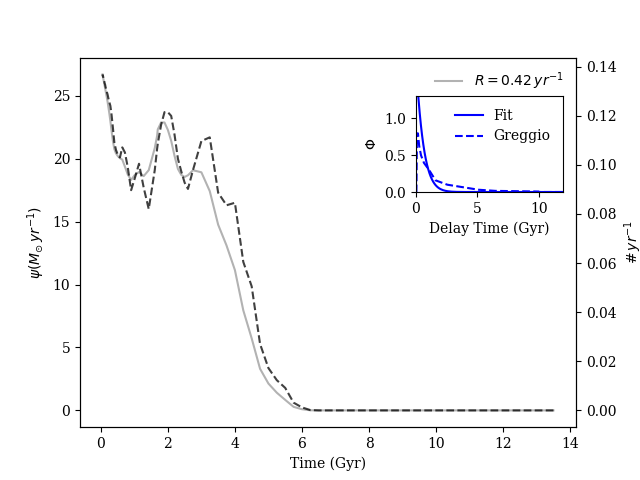
\includegraphics[width=4.5in]{Figure_2} 
   \caption{\footnotesize Example of best-fit delay-time distribution (inset) on the SFH of a sample host galaxy. }
   \label{fig:fg2}
\end{figure}

\section{discusssion}

\bibliography{strolger}{}

\begin{table}
    \centering
    \caption{Parameter Covariance MCMC SFD}
    \label{tab:parameter_covariance}
    \begin{tabular}{c|ccccc}
         & $f$ & $\xi$ & $\omega$ & $\alpha$ & $\log \phi$\\ 
        \hline
              $f$ &  0.41 & -125.69 &  6.61 & 33.98 & -0.41 \\ 
            $\xi$ & -125.69 & 412816.10 & -14898.10 & -52398.20 & 518.74 \\ 
         $\omega$ &  6.61 & -14898.10 & 660.60 & 2209.32 & -22.89 \\ 
         $\alpha$ & 33.98 & -52398.20 & 2209.32 & 27290.24 & -131.67 \\ 
        $\log \phi$ & -0.41 & 518.74 & -22.89 & -131.67 &  2.35 \\ 
        \hline
    \end{tabular}
\end{table}


\end{document}